\documentclass[12pt,letterpaper]{article}
\usepackage{fullpage}
\usepackage[top=2cm, bottom=4.5cm, left=2.5cm, right=2.5cm]{geometry}
\usepackage{amsmath,amsthm,amsfonts,amssymb,amscd}
\usepackage{lastpage}
\usepackage{enumerate}
\usepackage{fancyhdr}
\usepackage{mathrsfs}
\usepackage{xcolor}
\usepackage{graphicx}
\usepackage{listings}
\usepackage{hyperref}  
\usepackage{tikz}      
\usepackage{pgf}

\usepackage[scaled=0.85]{FiraMono}

\usetikzlibrary{arrows, automata}

\hypersetup{
    colorlinks=true,
    linkcolor=blue,
    linkbordercolor={0 0 1}
}
 
\newtheorem*{thm}{Theorem}

\renewcommand\lstlistingname{Algorithm}
\renewcommand\lstlistlistingname{Algorithms}
\def\lstlistingautorefname{Alg.}

\lstdefinestyle{Python}{
    language     = Python,
    aboveskip    = 3mm,
    belowskip    = 3mm,
    frame        = lines, 
    basicstyle   = \footnotesize\ttfamily,
    keywordstyle = \color{blue},
    stringstyle  = \color{green},
    commentstyle = \color{red}\small\ttfamily
}

\setlength{\parindent}{0.0in}
\setlength{\parskip}{0.05in}

% Edit these as appropriate
\newcommand\course{CSE 3500}
\newcommand\hwnumber{2}
\newcommand\NetIDa{mfm19005}

\pagestyle{fancyplain}
\headheight 35pt
\lhead{\NetIDa}
\chead{\textbf{\Large Homework \hwnumber}}
\rhead{\course \\ \today}
\lfoot{}
\cfoot{}
\rfoot{\small\thepage}
\headsep 1.5em

\begin{document}

\begin{center}
    \LARGE Problem Set
\end{center}

\section*{Problem 0}
\begin{center}
    \scalebox{0.455}{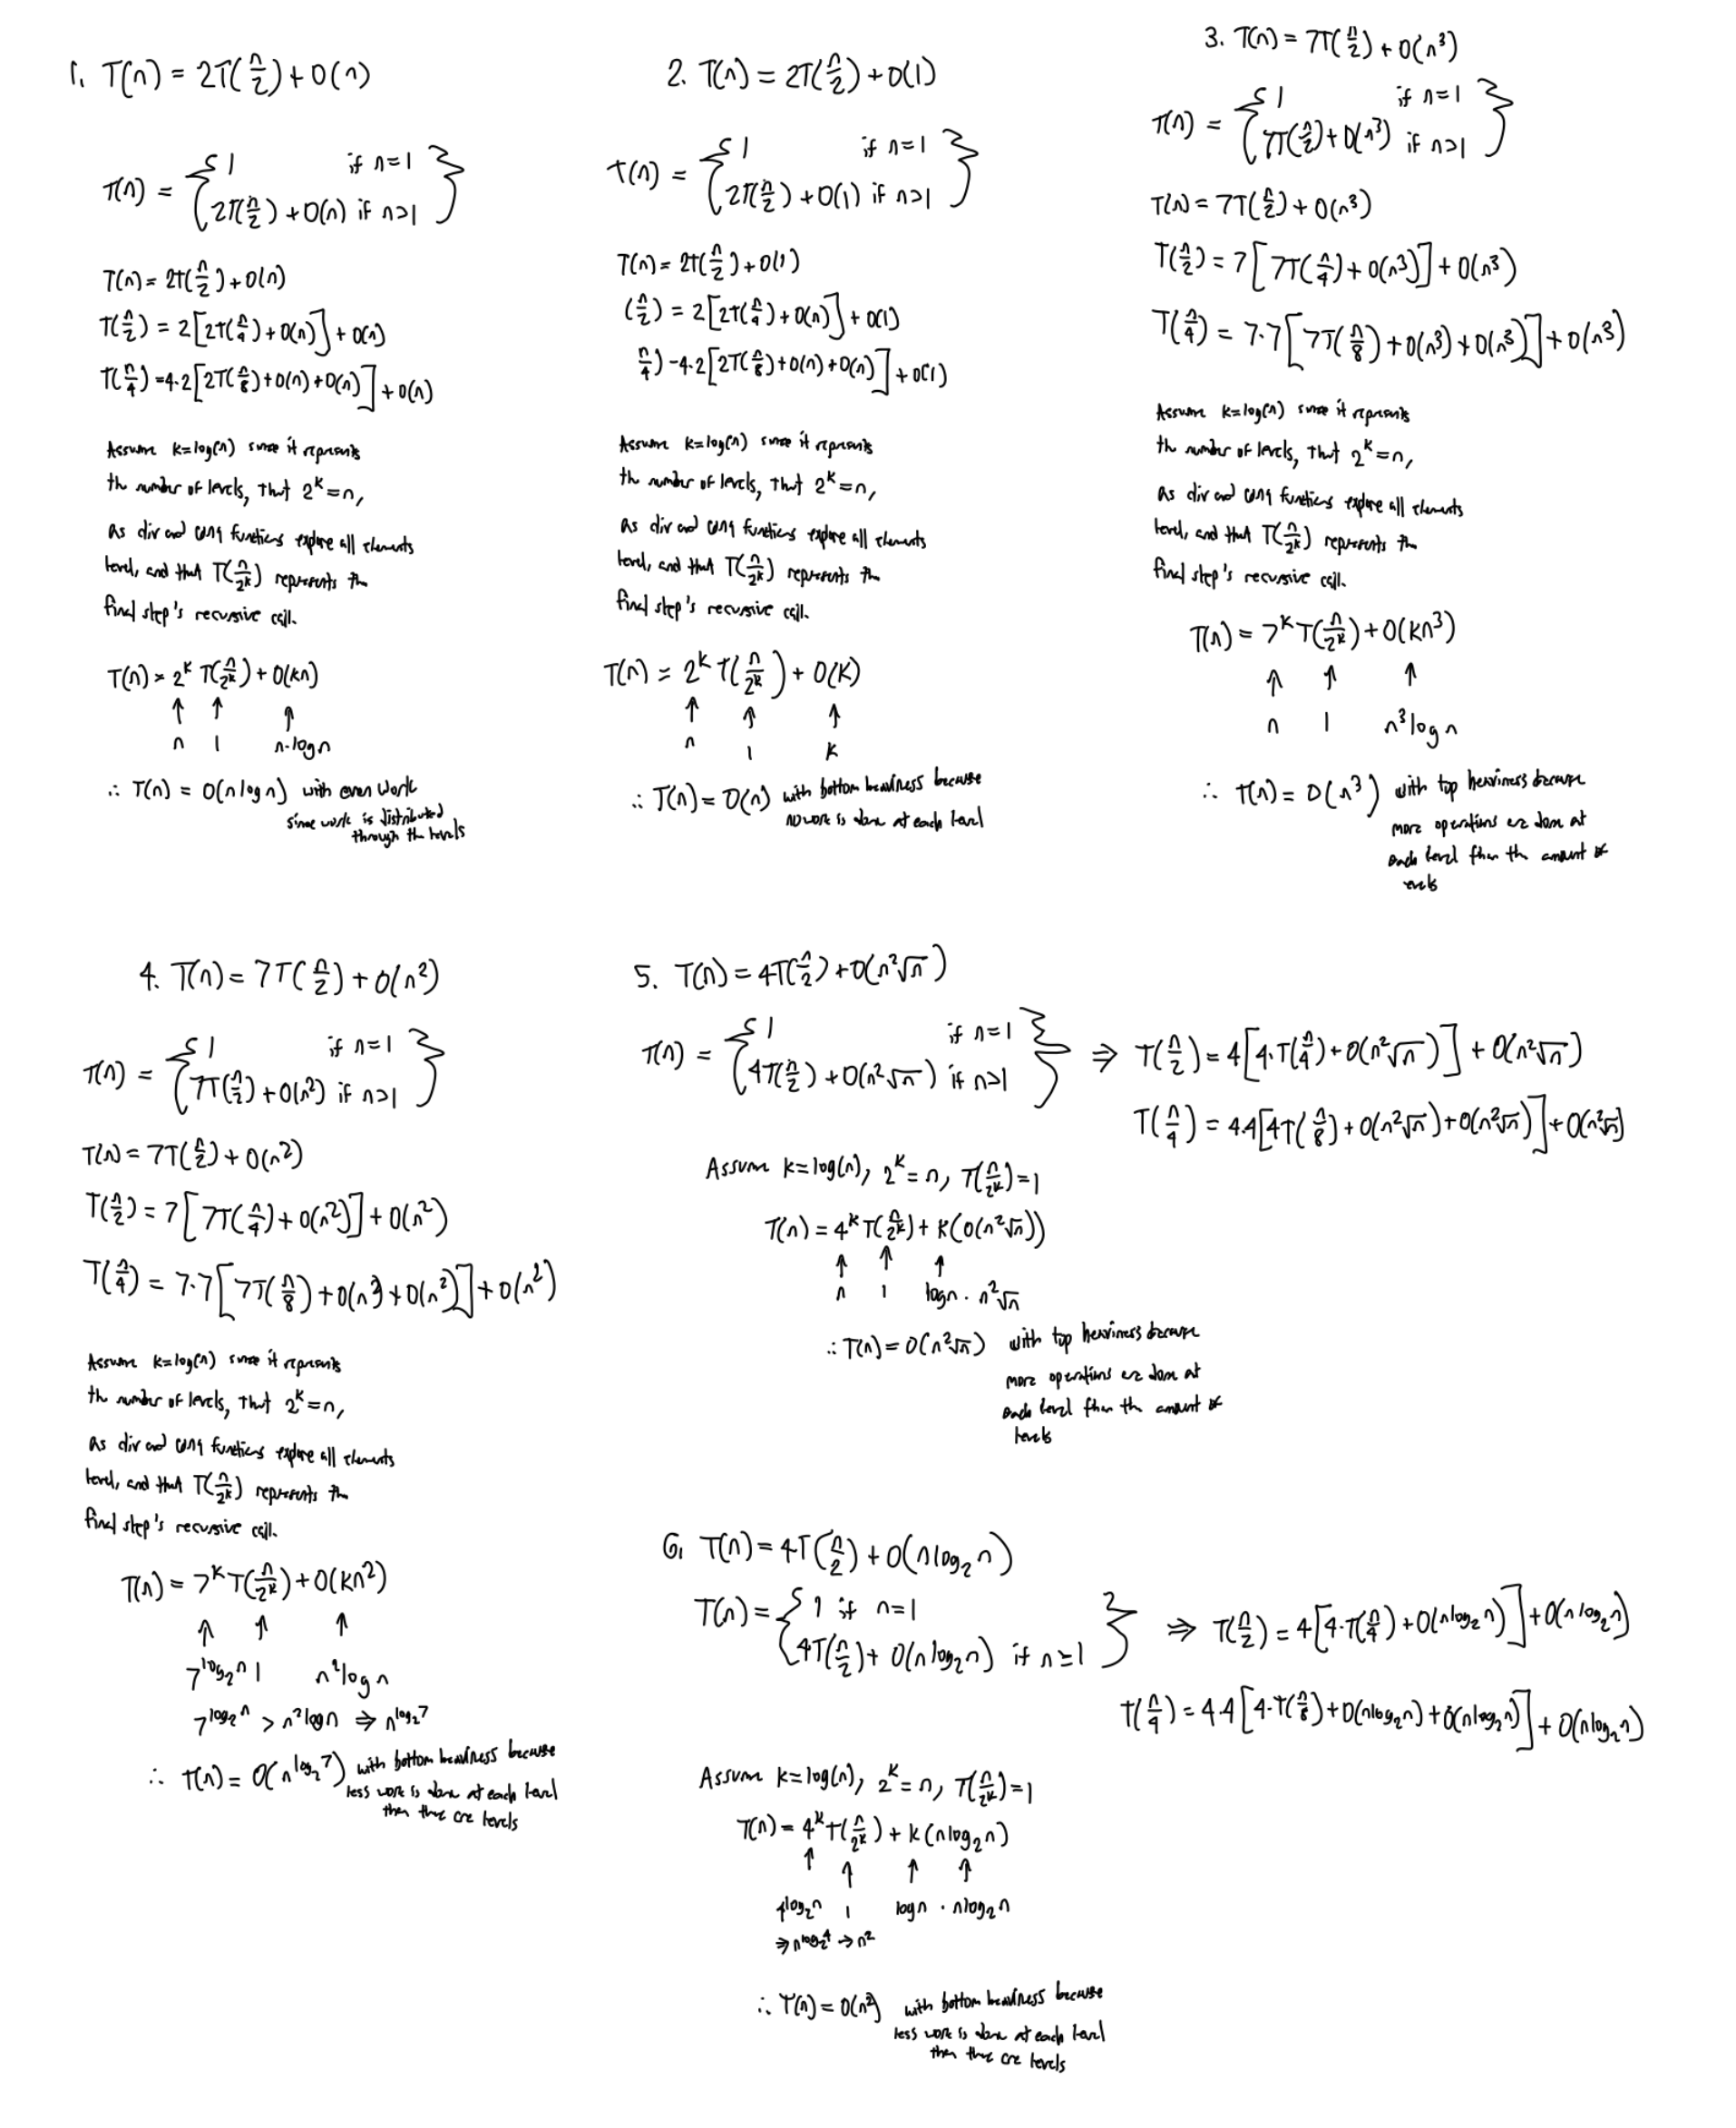
\includegraphics{problem0.png}}
\end{center}

\newpage
\section*{Problem 1}
You are given a $2^k * 2^k$ board of squares (e.g. a chess board) with the top left square removed. Prove, by giving a divide-and-conquer algorithm or argument, that you can exactly cover the entire board with L-shaped pieces (each covering 3 squares).

$\hfill \break$
We can feasibly show that any $2^k * 2^k$ chess board, with it's top left square removed can be filled by L-shaped pieces by defining an adequate base-case, and further by developing a strategy to traverse the board.

$\hfill \break$
Given this chess board, we can see that there are $(2^k * 2^k) - 1$ remaining pieces after removing the top-left piece. With this in mind, we can setup a base-case where $k = 1$, giving us a $2 * 2$ board. In this case, we can see that there are 3 remaining pieces, and thus we can fill the board with a singular L-shaped piece, in the only position it will fit.

$\hfill \break$
Now that we have a base-case setup, we can think about how we will split this board into smaller subproblems. Since this board will always have an even number of squares, we can split it into 4 equal quadrants. We can then recursively call our function on each of these quadrants, until we reach our base-case of a $2*2$ grid. When this base-case occurs, we will be able to fill the remaining board with the L-shaped piece we mentioned earlier. From this, we can re-merge the many $2*2$ grids back into the $2^k * 2^k$ grid, and as such we will have filled every possible space with an L-spaced piece.

$\hfill \break$
The specific algorithm we can use to accomplish this is outlined below, assuming we have a board with the top-left piece removed:
\begin{enumerate}
    \item If $k = 1$, fill the remaining three pieces of the board with an L-shaped piece, as this is our base-case.
    \item Otherwise, split the board into 4 equal quadrants, and recursively call our function on each of these quadrants.
    \begin{enumerate}
        \item Place an L-shaped piece in the middle of the partitioned board, and fill the remaining 3 pieces with L-shaped pieces.
        \item Repeat \textit{Step 2} and \textit{Step 2a} until the base-case is achieved.
    \end{enumerate}
\end{enumerate}

\newpage
\section*{Problem 2}
You are given an unsorted list L that has $k \geq 0$ pairs of indices $i < j$ such that $L[i] > L[j]$. These are called inverted pairs. Develop an $O(nlogn)$ algorithm that counts the number of inverted pairs (i.e. compute the value k).

$\hfill \break$
In order to count the number of inverted pairs in a list, we can use a divide-and-conquer approach using a variant of the classic merge sort algorithm. In this way, we will attain an $O(nlogn)$ runtime, and be able to leverage a simple recursive approach.

$\hfill \break$
To begin, we can recursively split the list in half into smaller sublists. This will be done until we reach a base-case of one item in each sorted list, in which case the sublist will be considered sorted. Now, instead of simply remerging all of the one-item sublists, we must keep the inversion property of this problem in mind. In this way, as we are remerging the sublists, we must check if $L[i] > L[j]$ for each $i$ and $j$ in the sublists. If this is the case, we can increment our counter by 1. Once we have remerged all of the sublists, we will have counted the number of inversions in the original list.

\newpage
\section*{Problem 3}
The \textit{best subset problem} is defined as, given a list $\left(x_1, x_2, ..., x_n\right)$ of integers (which can be positive, negative, or zero), find $(i, j)$ such that $x_i + x_{i+1} + ... + x_j$ is maximum for any
$1 \leq i \leq j \leq n$. For example, if $n = 10$ and the input is $\left(4, -8, -5, 8, -4, 3, 6, -3, 2, -11\right)$ then the output is $x_4 + x_5 + x_6 + x_7 = 8 - 4 + 3 + 6 = 13$.

\begin{enumerate}
    \item Develop an $O(n)$ algorithm for the related problem, best subset middle or BSM. The input to BSM is a list $\left(x_1, x_2, ... , x_n\right)$ of integers (which can be positive, negative, or zero) and the output is the maximum value of $x_i + x_{i+1} + ... + x_j$ such that $[i, j]$ spans $\frac{n}{2}$, in other words, for all possibilities for $i$ and $j$ such that $1 \leq i \leq \frac{n}{2} \leq j \leq n$.
    \item Design a recursive algorithm for the best subset problem with runtime $O(nlogn)$ that uses the BSM function.
    \item Argue that your algorithm is indeed correct and prove the runtime is $O(nlogn)$.
    \item (Extra credit: 5pts) Design an algorithm for the best subset problem that has $O(n)$ runtime. Argue why your algorithm is correct and has $O(n)$ runtime.
\end{enumerate}

In order to find the \textit{best subset middle}, we can use a dynamic programming approach in order to iterate through the array and compute the maximum subsets on each side. More specifically, we can split the given array into two, and then iterate through both the left and right hand sides of the split. Given these two subarrays, we can compute the maximal subsets for each. Knowing the maximum subset for each side, we can know compute along the middle which we split. In this way, we can see if the maximum of each subarray is between the split of the arrays.

$\hfill \break$
We are able to use recursion in order to divide and conquer this problem. With this in mind, we can implement a merge sort like algorithm which splits the original array into arrays of length one at the base case. Once they are fully split, we are able to merge them back together in such a way where we can compute the maximum subsets by keeping track of the maximums as they are being remerged.

$\hfill \break$
This algorithm must be $O(nlogn)$ since it constructed in the same way as a merge sort algorithm. If we compare what the two do, the merge sort algorithm arranges the subarrays it generates to be in order, while this algorithm looks through the subarrays in order to compute the maximum subsets. We can also break down the components of this recursive algorithm in order to prove that it must be $O(nlogn)$. This is because the splitting aspect of the algorithm runs in $O(logn)$ time for each level, and the computational aspect must check all $n$ items at each level. Therefore, the runtime must be $O(nlogn)$.


\end{document}
